\section{Linear Resource Usage Protocols}

\label{sec:protocols}

The \texttt{IO} type uses a
linear resource representing the current state of the outside world. But,
often, we need to work with other resources, such as files, network sockets,
or communication channels. In this section, we introduce an extension of
\texttt{IO} which allows creating and updating linear resources, and show how
to use it to implement a resource usage protocol for an automated teller
machine (ATM).

\subsection{Initialising Linear Values}

In QTT, multiplicities are associated with \emph{binders}, not with return
values or types. This is a design decision of QTT, rather than of Idris, and has
the advantage that we can use a type linearly or not, depending on
context. We can write functions that create values to be used linearly by
using \emph{continuations}, for example, to create a new linear array:

\begin{lstlisting}
newArray : (size : Int) -> (1 k : (1 arr : Array t) -> a) -> a
\end{lstlisting}

The array must be used exactly once in the scope of \texttt{k}, and if this is
the only way of constructing an \texttt{Array}, then all arrays are guaranteed
to be used linearly, so we can have in-place update. As a matter of taste, however, we may not want to write
programs with explicit continuations. Fortunately, \texttt{do} notation can
help; recall the bind operator for \TC{IO}:

\begin{lstlisting}
(>>=) : IO a -> (a -> IO b) -> IO b
\end{lstlisting}

This allows us to chain an IO action and its continuation, and \texttt{do}
notation gives syntactic sugar for translating into applications of
$\mathtt{>>=}$. Therefore, we can define an alternative $\mathtt{>>=}$
operator for chaining actions which return linear values. We will achieve
this by defining a new type for capturing interactive actions, extending
\texttt{IO}, and defining its bind operator.

\subsection{Linear Interactive Programs}

First, we define how many times the result of an operation can be used.
These correspond to the multiplicities $0$, $1$ and $\omega$:

\begin{lstlisting}
data Usage = None | Linear | Unrestricted
\end{lstlisting}

We declare a data type \TC{L}, which describes interactive programs that
produce a result with a specific multiplicity. We choose a short name \TC{L}
since we expect this to be used often:

\begin{lstlisting}
data L : {default Unrestricted use : Usage} ->
         Type -> Type where
\end{lstlisting}

In Section~\ref{sec:implicits} we described implicit arguments, which are
solved by unification. Here, \VV{use} is an implicit argument, and the
\texttt{default Unrestricted} annotation means that if its value cannot be
solved by unification, it should have a default value of \texttt{Unrestricted}.

\textbf{Aside:} \TC{L} is defined in a library \TC{Control.Linear.LIO},
distributed with Idris 2. In fact, its type is more general;
\texttt{L : (io : Type -> Type) -> \{use : Usage\} -> Type -> Type}. This
allows us to extend \emph{any} monad with linearity, not just \texttt{IO},
but this generality is not necessary for the examples in this paper.

Like \TC{IO}, \TC{L} provides the operators \TC{pure} and $\mathtt{>>=}$.
However, unlike \TC{IO}, they need to account for variable usage. One limitation
of QTT is that it does not yet support quantity polymorphism, so we must
provide separate \TC{pure} operators for each quantity:

\begin{lstlisting}
pure  : (  x : a) -> L         a
pure0 : (0 x : a) -> L {use=0} a
pure1 : (1 x : a) -> L {use=1} a
\end{lstlisting}

Idris translates integer literals using the \TC{fromInteger} function. We
have defined a \TC{fromInteger} function that maps \texttt{0} to
\DC{None} and \texttt{1} to \DC{Linear} which allows us to use integer
literals as the values for the \VV{use} argument.

The type of $\mathtt{>>=}$ is more challenging. In order to take advantage of
\texttt{do}-notation, we need a single $\mathtt{>>=}$ operator for chaining
an action and a continuation, but there
are several possible combinators of variable usage. Consider:

\begin{itemize}
\item The action might return an erased, linear or unrestricted value.
\item Correspondingly, the continuation must bind its argument at multiplicity
$0$, $1$ or $\omega$.
\end{itemize}

In other words, the type of the continuation to $\mathtt{>>=}$ depends on the
usage of the result of the action. We can therefore take advantage of
first-class types and \emph{calculate} the continuation type. Given the
usage of the action (\VV{u\_a}), the usage of the continuation (\VV{u\_k})
and the return types of each, \VV{a} and \VV{b}, we calculate:

\begin{lstlisting}
ContType : (u_a : Usage) -> (u_k : Usage) -> Type -> Type -> Type
ContType None u_k a b = (0 _ : a) -> L {use=u_k} b
ContType Linear u_k a b = (1 _ : a) -> L {use=u_k} b
ContType Unrestricted u_k a b = a -> L {use=u_k} b
\end{lstlisting}

Then, we can write a type for $\mathtt{>>=}$ as follows:

\begin{lstlisting}
(>>=) : {u_a : _} ->
        (1 _ : L {use=u_a} a) ->
        (1 _ : ContType u_act u_k a b) -> L {use=u_k} b
\end{lstlisting}

The continuation type is calculated from the usage of the first action, and is
correspondingly needed in the implementation, so \VV{u\_a} is run time
relevant. However, in practice it is removed by inlining.
Fortunately, the user of \TC{L} need not worry about these details. They
can freely use \texttt{do}-notation and let the type checker take care of
variable usage for them.

%, taking the type of $\>\>=$ to be one of:

%\begin{lstlisting}
%(>>=) : (1 _ : L {use=0} a) ->
%        (1 _ : (0 _ : a) -> L {use} b) -> L {use} b
%(>>=) : (1 _ : L {use=1} a) ->
%        (1 _ : (1 _ : a) -> L {use} b) -> L {use} b
%(>>=) : (1 _ : L a) ->
%        (1 _ : a -> L {use} b) -> L {use} b
%\end{lstlisting}

Finally, for developing linear wrappers for
\TC{IO} libraries, we allow lifting \TC{IO} actions:

\begin{lstlisting}
action : IO a -> L a
\end{lstlisting}

We use \FN{action} for constructing primitives. Note that we will not be
able to bypass any linearity checks this way, since it does not promise to
use the \TC{IO} action linearly, so we cannot pass any linear resources to
an \FN{action}. The implementation of \TC{L} is via a well-typed
interpreter~\cite{augustsson_exercise_1999}, a standard pattern in
dependently typed programming.

%We will return to the implementation of \TC{L} shortly, in
%Section~\ref{sec:implementl}. First, let us look at a small example of using
%\TC{L} to implement a state machine, with the transitions checked at
%compile time.

\subsection{Example: An ATM State Machine}

We can use linear types to encode the state of a resource, and implement
operations in \TC{L} to ensure that they are only executed when the resource is
in the appropriate state.  For example, an ATM should only dispense cash when a
user has inserted their card and entered a correct PIN. This is a typical
sequence of operations on an ATM:

\begin{itemize}
\item A user inserts their bank card.
\item The machine prompts the user for their PIN, to check the user is
entitled to use the card.
\item If PIN entry is successful, the machine prompts the user for an amount of
money, and then dispenses cash.
\end{itemize}

\begin{figure}[h]
\begin{center}
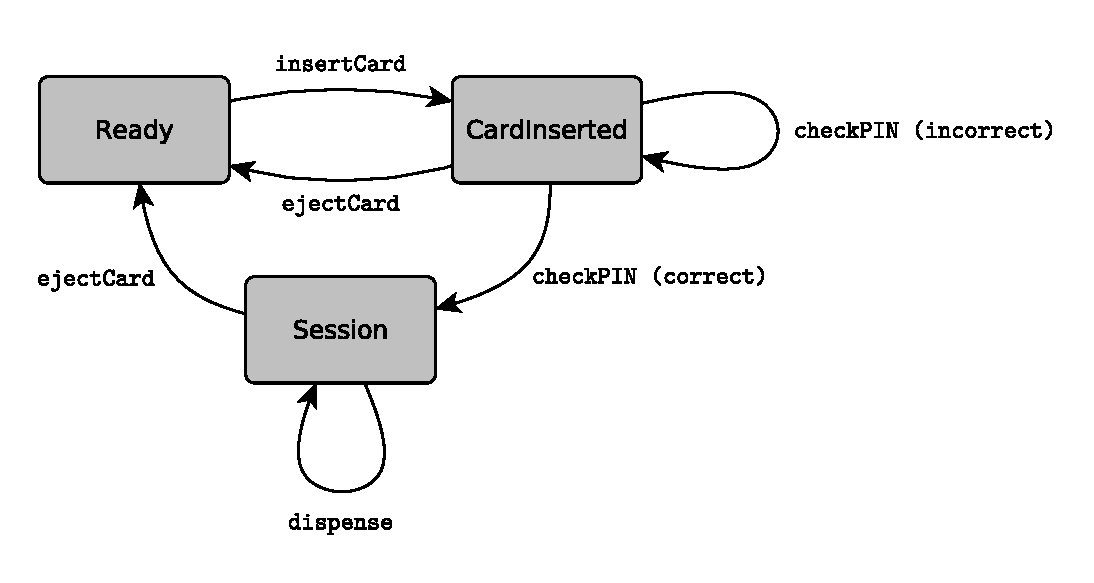
\includegraphics[width=10cm]{atm.pdf}
\end{center}
\caption{A state machine describing the states and operations on an ATM}
\label{fig:atm}
\end{figure}

Figure \ref{fig:atm} defines, at a high level, the states and operations on
an ATM, showing when each operation is valid. We will define these operations
as functions in the \TC{L} type, using a linear reference to a representation
of an ATM. We define the valid states of the ATM as a data type, then an
ATM type which is parameterised by its current state, which is one of:

\begin{itemize}
\item \DC{Ready}: the ATM is ready and waiting for a card to be inserted.
\item \DC{CardInserted}: there is a card inside the ATM but the PIN entry
is not yet verified.
\item \DC{Session}: there is a card inside the ATM and the PIN has been
verified.
\end{itemize}

\begin{lstlisting}
data ATMState = Ready | CardInserted | Session
data ATM : ATMState -> Type
\end{lstlisting}

We leave the definition of \TC{ATM} abstract. In practice, this is where we
would need to handle implementation details such as how to access and update a
user's bank account. For the purposes of this example, we are only interested
in encoding the high level state transitions in types.
%
We will need functions to initialise and shut down the reference:

\begin{lstlisting}
initATM  : L {use=1} (ATM Ready)
shutDown : (1 _ : ATM Ready) -> L ()
\end{lstlisting}

\begin{lstlisting}[caption={Operations on an ATM},label=atmops,float=h]
data HasCard : ATMState -> Type where
     HasCardPINNotChecked : HasCard CardInserted
     HasCardPINChecked : HasCard Session

data PINCheck = CorrectPIN | IncorrectPIN

insertCard : (1 _ : ATM Ready) -> L {use=1} (ATM CardInserted)
checkPIN : (1 _ : ATM CardInserted) -> (pin : Int) ->
           L {use=1}
             (Res PINCheck 
                  (\res => ATM (case res of
                                     CorrectPIN => Session
                                     IncorrectPIN => CardInserted)))
dispense : (1 _ : ATM Session) -> L {use=1} (ATM Session)
getInput : HasCard st => (1 _ : ATM st) ->
                         L {use=1} (Res String (const (ATM st)))
ejectCard : HasCard st => (1 _ : ATM st) -> L {use=1} (ATM Ready)
message : (1 _ : ATM st) -> String -> L {use=1} (ATM st)
\end{lstlisting}

\FN{initATM} creates a linear reference to an ATM in the initial state,
\TC{Ready}, which must be used exactly once. Correspondingly,
\FN{shutDown} deletes the linear reference.
Listing \ref{atmops} presents the types of the remaining operations, 
implementing the transitions from Figure \ref{fig:atm}.

Several details and design choices, are worthy of note. We have:
user-directed state transitions, where the
\emph{programmer} is in control over whether an operation succeeds;
general purpose operations, which do not change the state, and are part of
the machine's user interface; 
and,
machine-directed state transitions, where the \emph{machine} is in control
over whether an operation succeeds, for example the machine decides if PIN
entry was correct.

%. For example, only the machine knows,
%at run time, whether a PIN was entered successfully or not: this is the
%only way to enter the \DC{Session} state.

\paragraph*{User-directed state transitions}

The \FN{insertCard} card function takes a machine in the \DC{Ready} state,
and returns a new machine in the \DC{CardInserted} state. The type ensures
that we can only run the function with the machine in the appropriate state.
For \FN{dispense}, we need to satisfy the security property that the machine
can only dispense money in a validated session. Thus, it has an input state
of \DC{Session}, and the session remains valid afterwards.

For \FN{ejectCard}, it is only valid to eject the card if there is already
a card in the machine. This is true in \emph{two} states: \DC{CardInserted}
and \DC{Session}. Therefore, we define a \emph{predicate} on states which
holds for states where there is a card in the machine:

\begin{lstlisting}
data HasCard : ATMState -> Type where
     HasCardPINNotChecked : HasCard CardInserted
     HasCardPINChecked : HasCard Session
\end{lstlisting}

The type of \FN{ejectCard} then takes an input of type \TC{HasCard st},
which is a proof that the predicate holds for the machine's input state
\VV{st}.

\begin{lstlisting}
ejectCard : HasCard st => (1 _ : ATM st) -> L {use=1} (ATM Ready)
\end{lstlisting}

The notation \texttt{HasCard st => ...}, with the \texttt{=>} operator,
means that this is an \emph{auto implicit} argument. Like implicits,
and \texttt{default} implicits, these can be omitted. The type checker will
attempt to fill in a value by searching the possible constructors. In this
case, if \VV{st} is \DC{CardInserted}, the value will be
\DC{HasCardPINNotCheck}, and if it is \DC{Session}, the value will be
\DC{HasCardPINChecked}. Otherwise, Idris will not be able to find a value, and
will report an error.
%
Auto implicits are also used for interfaces,
corresponding to type classes in Haskell, although we do not use interfaces
elsewhere in this paper.

\paragraph*{General purpose operations}

The \FN{message} function displays a message to the user. Its type means that
we can display a message no matter the machine's state. Nevertheless, since an
ATM is linear, we must return a new reference. The \FN{getInput} function
reads input from the user, using the machine's keypad, provided that there
is a card in the machine. Again, this needs to return a new reference, along
with the input.
%
\TC{Res} is a \emph{dependent pair} type, where the first item is
unrestricted, and the second item is linear with a type computed from the
value of the first element. We describe this below in the context of
\FN{checkPIN}.

\paragraph*{Machine-directed state transitions}

The most interesting case is \FN{checkPIN}. In the other functions, the
programmer is in control of when state transitions happen, but in this case,
the transition may or may not succeed, depending on whether the PIN is
correct. To capture this possibility, we return the result in a dependent
pair type, \TC{Res}, defined as follows in the Idris Prelude:

\begin{lstlisting}
data Res : (a : Type) -> (a -> Type) -> Type where
     (#) : (val : a) -> (1 r : t val) -> Res a t
\end{lstlisting}

This pairs a value, \VV{val}, with a linear resource whose type is computed
from the value. This can be illustrated with a partial ATM program:

\begin{lstlisting}
runATM : L ()
runATM = do m <- initATM
            m <- insertCard m
            ok # m <- checkPIN m 1234
            ?whatnow
\end{lstlisting}

This program initialises an ATM, inserts a card, then checks whether the card
has the PIN 1234. Checking the PIN returns a \TC{Res}, which we deconstruct,
then we can inspect the hole \texttt{?whatnow} to see where to go from here:

\begin{lstlisting}
   ok : PINCheck
 1 m : ATM (case ok of { CorrectPIN => Session
                         IncorrectPIN => CardInserted })
------------------------------
whatnow : L ()
\end{lstlisting}

So, we have the result of the \TC{PINCheck}, and an updated \TC{ATM}, but
we will only know the state of the \TC{ATM}, and hence be able to make
progress in the protocol, if we actually check the returned result!
We cannot know statically what the next state of the machine is
going to be, but using first class types, we \emph{can} statically check that the
necessary dynamic check is made.
%
We could also use a sum type, such as \TC{Either}, for the
result of the PIN check, e.g. 

\begin{lstlisting}
checkPIN : (1 _ : ATM CardInserted) -> (pin : Int) ->
           L {use=1} (Either (ATM CardInserted) (ATM Session))
\end{lstlisting}

This would arguably be simpler. On the other hand, by returning an \texttt{ATM}
with an as yet unknown state, we can still run operations on the \texttt{ATM}
such as \FN{message} even before resolving the state. This might be useful
for diagnostics, or for user feedback, for example.
Listing~\ref{atmrun} shows one possible ATM protocol implementation, displaying
a message before checking the PIN, then dispensing cash if the PIN was valid.
Note that the protocol also requires the card to have been ejected before
the machine is shut down.

\begin{lstlisting}[caption={Example ATM protocol implementation},label=atmrun,float=h]
runATM : L ()
runATM = do m <- initATM
            m <- insertCard m
            ok # m <- checkPIN m 1234
            m <- message m "Checking PIN"
            case ok of
                 CorrectPIN => do m <- dispense m
                                  m <- ejectCard m
                                  shutDown m
                 IncorrectPIN => do m <- ejectCard m
                                    shutDown m
\end{lstlisting}

\textbf{Aside:} Linearity and exceptions do not mix well, since when we
catch an exception, we need to know what state the machine was in at the point
it was thrown in order to clean up effectively. On the other hand, if we have
to check every result as in Listing~\ref{atmrun}, we will end up with a lot
of nested \texttt{case} blocks, which are hard to read. As a compromise,
Idris provides a pattern matching bind notation~\cite{brady_tfp14}, which
allows us to code to a ``happy path'' and deal with alternatives as they
arise. For example:

\begin{lstlisting}
runATM : L ()
runATM = do m <- initATM
            m <- insertCard m
            CorrectPIN # m <- checkPIN m 1234
               | IncorrectPIN # m => ?failure
            ?success
\end{lstlisting}

The ``happy path'' is that the PIN was entered correctly. The alternative
we need to handle is the \DC{IncorrectPIN} case.

%\subsection{Implementing \TC{L}}

%\label{sec:implementl}
